\documentclass[14pt,a4paper]{extreport}
\usepackage[a4paper, left=2cm, right=2cm, top=1cm, bottom=2cm]{geometry}

\usepackage{listings} 
\usepackage{caption}
\usepackage{graphicx} % Для того, чтобы вставлять картинки.
\usepackage{wrapfig} % Картинка, обтекаемая текстом.
\usepackage{amssymb}
\usepackage{amsmath} % Чтобы вставлять обычный текст в формулу с помощью \text.

\usepackage{multicol} % Для написания текста в несколько колонок

\usepackage{setspace} % Для изменения межстрочного интервала внутри текста. \begin{spacing}{0.8}.

\usepackage{float}   % Чтобы была опция таблиц H, запрещающая им бегать по документу
\restylefloat{table}

\usepackage{gensymb} % Геометрические символы. (градусы \degree)..

\usepackage[warn]{mathtext} % Русские символы в формулах. Нужно писать до пакета babel. Указывает, что в формулах используются символы кириллицы, которые по умолчанию печатаются прямым шрифтом.

\usepackage[T2A]{fontenc} % Установить кодировку шрифта для отображения кириллицы в формулах.
\usepackage[utf8]{inputenc}

\usepackage[russian]{babel} % Для переноса текста. Нельзя указывать одновременно russian и english, так как использует язык, который стоит правее.

\usepackage{indentfirst} % Красная строка в первом абзаце.

\usepackage{comment} % Для многострочный комментариев.
\setlength{\parindent}{1.25cm} % Отступ красной строки

\linespread{1.25} % Межстрочный интервал. По умолчанию 1.0

\DeclareSymbolFont{T2Aletters}{T2A}{cmr}{m}{it} % Сделать так, чтобы кириллица в формулах печаталась курсивом

% Объявляем новую команду для переноса строки внутри ячейки таблицы
\newcommand{\specialcell}[2][c]{%
	\begin{tabular}[#1]{@{}c@{}}#2\end{tabular}}

\begin{document}
	
	\begin{center}
		\large
		\textsc{Лабораторная работа №2.2.3}
		
		\LARGE
		\textbf{\textsc{Исследование осмотического давления}}
		\\[5mm]
		
		\large
		Маслов Артём\\
		Брицко Владимир\\
		Б01-104
		\\[3mm]
		18.05.2022
	\end{center}
	
	\textbf{\large Цель работы:}
	
	\begin{enumerate}
		\item Измерение осмотического давления при разной концентрации жёлтой кровяной соли;
		\item Проверка закона Вант-Гоффа.
	\end{enumerate}
	
	\textbf{\large Оборудование:}
	
	Осмометр; секундомер; пипетка; мерный стаканчик; химический стакан.
	
	\textbf{\Large Аннотация}

В работе изучаются свойства полупроницаемых перегородок. Измеряется осмотическое давления при разной концентрации кровяной соли. 

\textbf{\Large Теория}

\textit{Полупроницаемой перегородкой} называется перегородка, которая пропускает молекулы растворителя, но не пропускает молекулы растворённых в ней соединений. Прохождение растворителя через полупроницаемую перегородку называется \textit{осмосом}.


	
	

\textbf{\Large Схема экспериментальной установки}

Схема используемого в работе осмометра приведена на рисунке:

\begin{figure}[H]
	\centering
	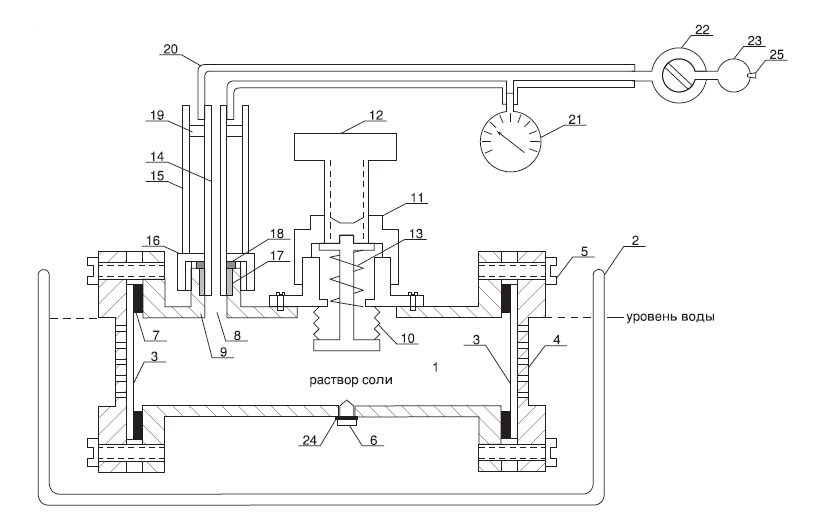
\includegraphics[width=1 \textwidth]{../images/scheme_experiment.png}
\end{figure}

\begin{multicols}{2}
	\begin{spacing}{0.3}
		\begin{enumerate}
			\item Контейнер для раствора соли.
			\item Сосуд с дистиллированной водой.
			\item Целлофановая плёнка.
			\item Защитная сетка.
			\item Прижимной винт.
			\item Пробка-отверстие для заполнения сосуда раствором;
			\item Резиновая прокладка.
			\item Отверстие, через которое раствор поступает в капилляр.
			\item Металлическая втулка, запрессованная в корпус контейнера.
			\item Гофрированная поверхность.
			\item Накидная гайка для грубой регулировки объёма сосуда.
			\item Винт тонкой регулировки объёма.
			\item Пружина.
			\item Стеклянный капилляр.
			\item Металлический кожух капилляра.
			\item Накидная гайка кожуха.
			\item Резиновая трубка, герметизирующая прокладка.
			\item Металлическая шайба.
			\item Подвижная резиновая втулка для крепления капилляра.
			\item Резиновый шланг.
			\item Манометр.
			\item Стеклянный кран.
			\item Резиновая груша для создания повышенного внешнего давления.
			\item Клапан.
		\end{enumerate}
	\end{spacing}

\end{multicols}
	
\newpage
	
Раствор заливается в контейнер 1, который помещается в сосуд с растворителем 2. Контейнер представляет собой куб, закрытый с четырёх сторон полупроницаемыми целлофановыми мембранами 3 толщиной $0,2$ мм. Мембраны зажимаются между стенками куба и металлическими сетками 4, которые предохраняют мембраны от раздувания наружу. Между мембранами и стенками вставлены резиновые уплотнения 7. Сосуд заполняется раствором через отверстие в дне куба, плотно закрываемое металлической гайкой 6 с резиновой прокладкой 21. Через крышку куба вставлен стеклянный капилляр 14, внутренний диаметр $0,5$ мм.

В процессе осмоса объём раствора увеличивается, и уровень раствора движется по капилляру вверх. Скорость подъёма уменьшается при избыточном давлении воздуха на верхнем конце капилляра. Избыточное давление создаётся с помощью груши 23 со встроенный клапаном 25 и фиксируется краном 22. Давление измеряется манометром 21. Кран 22 также позволяет сбросить избыточное давление.

На крышке куба смонтировано устройство, состоящее из гофра 10, накидной гайки 11, винта 12 и пружины 13, позволяющие менять объём внутреннего пространства в кубе. Это бывает необходимо, если в процессе опыта мембраны вытягиваются и уровень раствора в капилляре понижается. При закручивании винта 12 объём контейнера уменьшается и раствор вытесняется в капилляр. Таким образом, уровень раствора можно установить на удобной для наблюдения высоте.




	
	\textbf{\Large Описание эксперимента}

В работе измеряется осмотическое давление водного раствора жёлтой кровяной соли $K_4 Fe (CN)_6$, при нескольких значениях концентрации и проверяется справедливость закона Вант-Гоффа.

Молекулы жёлтой кровяной соли при растворении диссоциируют:
$$
K_4 Fe (CN)_6 \rightarrow 4 K^+ + [Fe (CN)_6]^{4-}
$$

Ионы $K^+$ свободно проникают через используемую в работе перегородку и не создают осмотическое давление.
	
	\textbf{\Large Вывод}

В работе наблюдался прямой и обратный осмос, было измерено осмотическое давление при разной концентрации раствора.

\begin{tabular}{|c|c|c|}
	\hline
	$n$, $\%$ & $P_{осм}$, Па & $P_{выч}$, Па \\
	\hline
	$0,300 \%$ & $9,6 \pm 0,6$  & $20,2$ \\
	$0,150 \%$ & $7,5 \pm 3,0$  & $10,1$ \\
 	$0,075 \%$ & $6,0 \pm 0,4$  & $5,0$  \\
	\hline
\end{tabular}

Проверить закон Вант-Гоффа не удалось, измеренное осмотическое давление не совпадает с вычисленным. Сложно определить, является ли зависимость $P_{осм}$ линейной, так как для этого нужно проводить измерения при большем числе концентраций.

На результат эксперимента могли повлиять следующие факторы:

\begin{enumerate}
	\item Во время измерений было обнаружено падение давления в системе на $\approx 7$ делений манометра.
	\item Полупроницаемые перегородки давно не менялись и со временем могли засориться, что приводит к понижению измеренного давления от вычисленного по формуле Вант-Гоффа. 
\end{enumerate}
	
\end{document}